\documentclass{documentation}
\usepackage{tikz}
\usetikzlibrary{shapes.geometric, arrows}
\tikzstyle{module} = [rectangle, rounded corners, minimum width=3cm, minimum height=1cm,text centered, draw=black]

\begin{document}

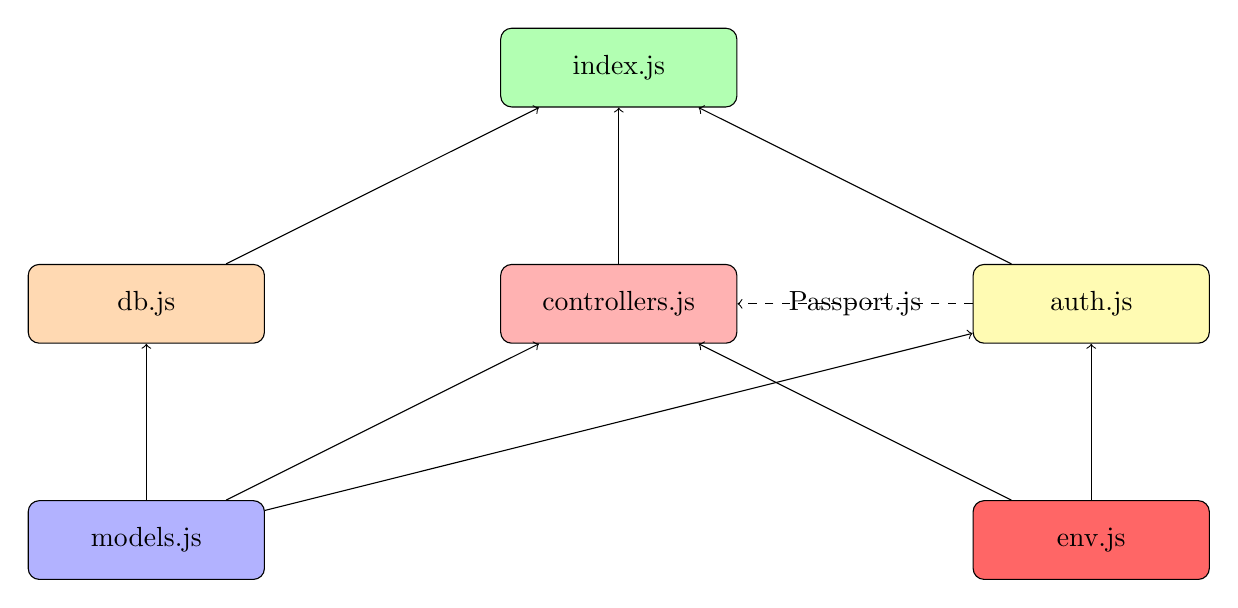
\begin{tikzpicture}[node distance=3cm]
    \node[module, fill=green!30] (index) {index.js};

    \node[module, fill=orange!30, below of=index, xshift=-6cm] (db) {db.js};
    \node[module, fill=blue!30, below of=db] (models) {models.js};
    
    \node[module, fill=red!30, below of=index, xshift=0] (controllers) {controllers.js};

    \node[module, fill=yellow!30, below of=index, xshift=6cm] (auth) {auth.js};
    \node[module, fill=red!60, below of=auth] (env) {env.js};

    
    \draw [->] (db) -- (index);
    \draw [->] (controllers) -- (index);
    \draw [->] (auth) -- (index);
    \draw [dashed, ->] (auth) -- node[anchor=center]{Passport.js} (controllers);
    \draw [->] (env) -- (auth);
    \draw [->] (env) -- (controllers);
    \draw [->] (models) -- (db);
    \draw [->] (models) -- (auth);
    \draw [->] (models) -- (controllers);

\end{tikzpicture}

\end{document}